\chapter{Optimization}
\section{Introduction}
The main goal of the project is to have the car consume the least amount of fuel
possible. In the ideal world should the engines and motors therefore always operate
within a certain the range of their optimal point of operation. The torque request
from each of the engine/motors should be with this goal in mind in order to reduce
fuel consumption. In addition to this goal, there is a number of constraints that
needs to be considered on top of this generic optimization.  Things like track
topography, super-capacitor voltage, competitors on the track etc will all weigh in
on the output request. The optimization algorithm used ELBA was developed as a part
of a Master Thesis~\cite{liu2016}. The control architecture for ELBA consists of a
two or three layers and the thesis have completed the top layer speed reference
control. This chapter will cover the decentralized hierarchical predictive control
that is used to calculate the speed trajectory.

\section{Constraints}
The optimization is limited by the constraints of the physical system, meaning that
the controller is not able to operate outside the limits of the system. These limits
are,
\begin{align}
    &U_{cap} \in [39,48]~\textup{V} \\
    &\nu \in [0,15]~\textup{m/s}\\
    &a_{\max} \in [-1,1]~\textup{m/s$^2$}
\end{align}
where $U_{cap}$ is the voltage level of the super-capacitor, $\nu$ is the speed and
$a$ is the acceleration in every time step. Due to the fact that there is a lower
limit to the voltage level of the super-capacitor, it is necessary to change drive
mode to the ICE in order to regenerate and store energy until the upper limit is
reached. Since the optimization is currently only done in the top layer, there
is a need for the voltage limit to be considered manually in the model.

\section{Simulink implementation}
The complete description of the algorithm is found in~\cite{liu2016} and the
implementation is based on this thesis.
\begin{figure}[H]
    \centering\label{fig:optimization_cont}
    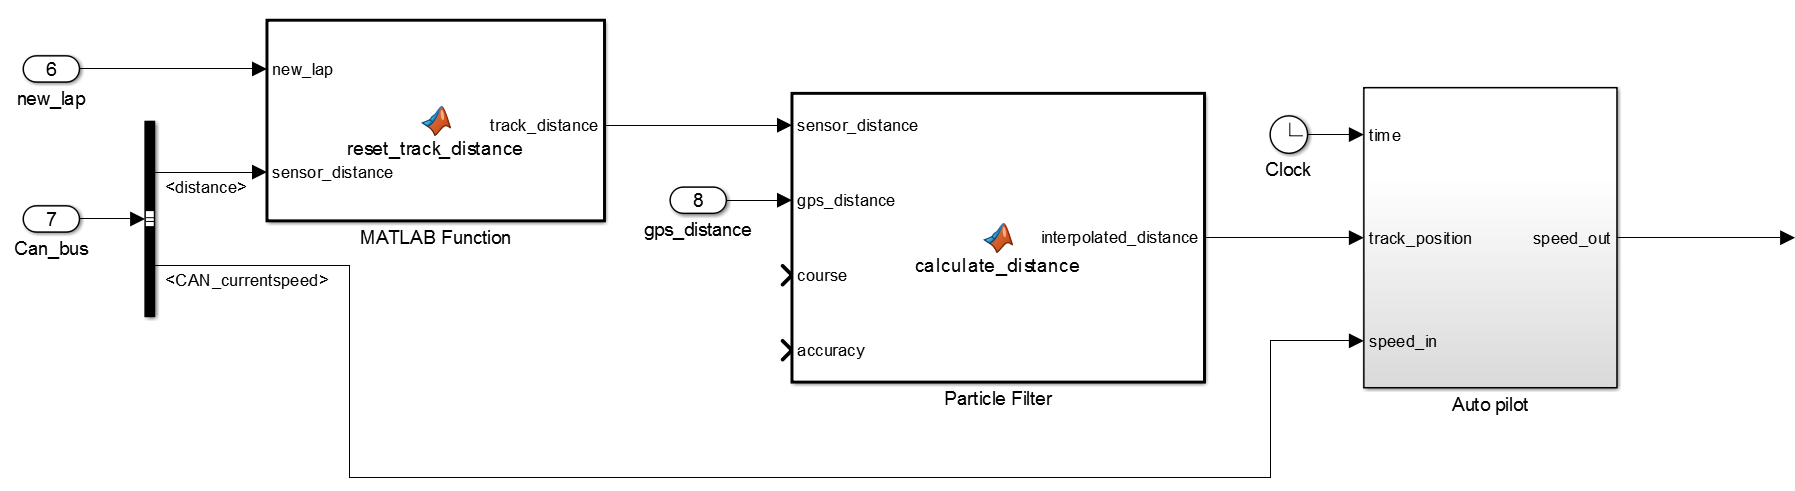
\includegraphics[width=\textwidth]{./img/optimization_cont.png}
    \caption{Simulink implementation for the Hierarchal Optimization Algorithm}
\end{figure}
In Figure~\ref{fig:optimization_cont} the function
\textit{reset\_track\_distance} takes an absolute dead reckoning position
calculated from the shaft encoder and an indicator for a new
lap,~\textit{new\_lap} as input. When the indicator for a new lap is pressed,
the dead reckoning position is zeroed in the function block and the position is
calculated and delivered as output. The position is sent to a Particle Filter
block where both the dead reckoning and the GPS position is supposed to be used
to get the estimation of which point of the discretized track the car is closest
to. However, the Particle Filter itself is not implemented at the moment and is
considered to be something future groups need to work on. 

\section{Position recognition}
The optimization bases the output reference speed on the current position on the
track. This yields the need for a position recognition with an accuracy precise
enough to be able filter it with sufficient results. The track itself, rather
then time is discretized in order to get a more accurate position in relation to
the tracks topography. \\
There is two ways of finding ELBAs positon on the track. The first way is a dead
reckoning system based on the shaft encoder~\cite[p.~49]{elba2015},
which calculates the position based on the rotational speed of the shaft. The
second way is based on the GPS system implemented in the race capture pro 2,
where the GPS signal is taken from it's raw form and reshaped with a
Lua-script\footnote{Lua is a dynamically typed scripting language, www.lua.org}
into a CAN-message that is sent on the CAN-bus.
